\documentclass[12pt]{article}
\usepackage[a4paper, margin=.30in]{geometry}
%\usepackage{array}
\usepackage{fancybox}

\usepackage{graphicx, subfig, wrapfig, makecell,multirow }
\newcommand\headerMe[2]{\noindent{}#1\hfill#2}
\renewcommand \thesection{\Roman{section}}

\newcolumntype{M}[1]{>{\raggedright}m{#1}}




\begin{document}

\begin{center}


	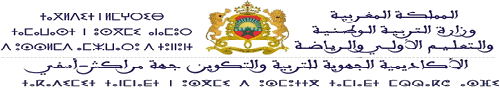
\includegraphics[width=0.66\textwidth]{./img/logo_arefmsoct2021.png}
\end{center}

%\headerMe{Royaume du Maroc}{année scolaire \emph{2022-2023}}\\
%\headerMe{Ministère de l'Éducation nationale, }{  }\\
%\headerMe{du Préscolaire et des Sports}{Établissement : \emph{Lycée SKHOR qualifiant}}\\

\begin{center}
%Devoir surveillé N°1 \\
%Durée 2h00\\
\underline{2-BAC Section des sciences expérimentales: Option de sciences physiques}\\

    \vspace{.2cm}
\hrulefill
\Large{Physique-Chimie}
\hrulefill\\
\end{center}
%end Headerss------------------------


%__________________Chimie ______________________-
%%%%%%%+_+_+_+_+_+_+_+_+_Partie1
%\section[A]{Introduction }
 \begin{center}
\begin{tabular}{|c|c|c|c|c|c|}
\hline
     \multicolumn{6}{||c||}{\bf{Exercice 1 : Propagation des ondes} }\\\hline
	 \makecell{domaine\\de la \\question}&Q	& \makecell{Référence de la question
 dans le cadre de référence } &\makecell{La difficulté\\de la\\question} & \makecell{Estimation \\du \\temps } & \makecell{Champ\\couvert\\par\\le sujet} \\\hline

	%
 \multirow{4}{*}{Les Ondes}&1.1 & Définir une onde mécanique& 90\%& 5min &  \\\cline{2-5}

							&1.2&\makecell{Définir une onde transversale et une \\onde longitudinale} & 85\%& 5min & \\\cline{2-5}

 &1.3 & \makecell{Connaître les caractéristiques de l’onde lumineuse} &85\% & 5min & \\\cline{2-5}
 & 2.1& \makecell{Exploiter la relation entre le retard temporel,\\la distance
et la célérité.}&70\% & 8min& 70\% \\\cline{2-5} 
				& 2.2& \makecell{Exploiter des documents expérimentaux et
\\des données pour déterminer la vitesse }& 70\% &8min&\\\cline{2-5}
										  &2.3& \makecell{Calculer la valeur du retard temporel} & 90\% & 3min&\\\hline

\end{tabular}
\end{center}


 \begin{center}
\begin{tabular}{|c|c|c|c|c|c|}
\hline
     \multicolumn{6}{||c||}{\bf{Exercice 2 : LES SYSTÈMES ÉLECTRIQUES} }\\\hline
     \multicolumn{6}{||c||}{\bf{Partie 1 : la réponse d’un dipôle RC} }\\\hline
	 \makecell{domaine\\de la \\question}&Q	& \makecell{Référence de la question
 dans le cadre de référence } &\makecell{La difficulté\\de la\\question} & \makecell{Estimation \\du \\temps } & \makecell{Champ\\couvert\\par\\le sujet} \\\hline

 Electricité	&1.1 &\makecell{ Représenter les tensions électrique et\\Reconnaître le phénomène de la charge\\ d'un condensateur} & 50\% & 2min&\\\cline{2-5}

				&1.2&\makecell{Etablir l’équation différentielle lorsque le dipôle \\RC est soumis à un échelon de tension.} &80\% & 3min & \\\cline{2-5}

				&1.3&\makecell{ vérifier la solution de l’équation différentielle\\lorsque le dipôle \\RC est soumis à un échelon de tension.} & 60\% & 2min & 50\% \\\cline{2-5}

				&1.4&\makecell{Connaitre et exploiter l’expression de la constante\\ du temps} &80\%& 2min & \\\cline{2-5}
				&1.5&\makecell{exploiter l’expression de la constante\\ du temps} &80\%& 2min & \\\hline
			\end{tabular}
\end{center}

 %
 \begin{center}
\begin{tabular}{|c|c|c|c|c|c|}
\hline
     \multicolumn{6}{||c||}{\bf{Partie 2 : la réponse d’un dipôle RL} }\\\hline
	 \makecell{domaine\\de la \\question}&Q	& \makecell{Référence de la question
 dans le cadre de référence } &\makecell{La difficulté\\de la\\question} & \makecell{Estimation \\du \\temps } & \makecell{Champ\\couvert\\par\\le sujet} \\\hline

	& 2.1& \makecell{mis en évidence retard à l’établissement\\du courant,déterminer L’élément\\du circuit responsable de ce phénomène  } & 50\% & 2min &\\\cline{2-5}

 Electricité&2.2& \makecell{Déterminer l’expression de l'intensité du\\courant $i(t)$ lorsque le dipôle RL est soumis à \\un échelon de
tension et en déduire l’expression \\de la tension aux
bornes de la \\bobine et aux bornes du conducteur
ohmique.} & 30\% & 4min & 50\% \\\cline{2-5}


		  &2.3& \makecell{Reconnaître et représenter les courbes de variation,
\\en fonction du temps, de l'intensité du courant
$i(t)$
\\passant dans la bobine et les grandeurs \\qui lui sont
liées et les exploiter.} & 30\% & 3min & \\\cline{2-5}

						 &2.4& \makecell{Connaître et exploiter l'expression \\de la constante de
temps.}& 80\%&2min& \\\cline{2-5} 

						 &2.5& \makecell{Connaître et exploiter l'expression \\de la constante de
temps.}& 80\%&2min& \\\hline 
\end{tabular}
\end{center}


\begin{center}
\begin{tabular}{|c|c|c|c|c|c|}
\hline
     \multicolumn{6}{||c||}{\bf{Partie 3 : la réponse d’un dipôle RLC} }\\\hline
	 \makecell{domaine\\de la \\question}&Q	& \makecell{Référence de la question
 dans le cadre de référence } &\makecell{La difficulté\\de la\\question} & \makecell{Estimation \\du \\temps } & \makecell{Champ\\couvert\\par\\le sujet} \\\hline

 Electricité	&3.1 &\makecell{Exploiter des documents expérimentaux pour \\reconnaitre les régimes d’amortissement  } & 90\% & 3min&\\\cline{2-5}

 &3.2 &\makecell{Etablir l’équation différentielle pour la tension
\\aux bornes du condensateur } & 70\% & 6min&\\\cline{2-5}

 &3.3 &\makecell{Connaître et exploiter l'expression \\de la période
propre. } & 50\% & 2min& 50\%\\\cline{2-5}


 &3.4 &\makecell{Connaître la méthode entretenir \\les oscillations en apportant de l’énergie \\au système grâce à un dispositif qualifié de \\"montage à résistance négative ".  } & 60\% & 2min&\\\hline


\end{tabular}
\end{center}



\begin{center}
\begin{tabular}{|c|c|c|c|c|c|}
\hline
     \multicolumn{6}{||c||}{\bf{Exercice 3 : Mécanique} }\\\hline
     \multicolumn{6}{||c||}{\bf{Partie A } }\\\hline
	 \makecell{domaine\\de la \\question}&Q	& \makecell{Référence de la question
 dans le cadre de référence } &\makecell{La difficulté\\de la\\question} & \makecell{Estimation \\du \\temps } & \makecell{Champ\\couvert\\par\\le sujet} \\\hline

 Mécanique	&1 &\makecell{Connaitre et exploiter les expressions du \\vecteur vitesse et de la position
 }& 40\% & 6min&\\\cline{2-5} 
	 	&2 &\makecell{trouver l’équation de la trajectoire et établir \\les
expressions de la portée et la \\flèche et les
exploiter. } & 90\% & 5min&\\\cline{2-5}
 \multicolumn{6}{||c||}{\bf{Partie B} }\\\cline{2-5}
	
 Mécanique	&1.1 &\makecell{
	 Etablir l’expression de la période propre du
\\pendule pesant.
}& 50\% & 5min&\\\cline{2-5} 

		&1.2 &\makecell{
 Connaître et exploiter l’expression de la
\\période propre et la fréquence propre du pendule
\\dans le cas des petites oscillations.
		}& 50\% & 5min&\\\cline{2-5} 

		&2.1 &\makecell{
	Appliquer la relation fondamentale de la
\\dynamique à un pendule de torsion pour établir
\\l’équation différentielle
		}& 90\% & 6min&\\\cline{2-5} 

		&2.1 &\makecell{
-Connaître et exploiter l'expression de l'énergie
\\mécanique du pendule de torsion.
%Déterminer la nature du mouvement du pendule
%\\de torsion, écrire et exploiter les équations du
%mouvement
		}& 60\% & 8min& 40\%\\\cline{2-5} 

		&2.2 &\makecell{
-Connaître et exploiter l'expression de l'énergie
\\mécanique du pendule \\de torsion et le Travail d'une force.
%Déterminer la nature du mouvement du pendule
%\\de torsion, écrire et exploiter les équations du
%mouvement
		}& 40\% & 8min&\\\cline{2-5} 

		&2.3 &\makecell{
		Exploiter la conservation et la non-conservation
\\de l'énergie mécanique du pendule de torsion.
		}& 40\% & 5min&\\\hline 






\end{tabular}
\end{center}


\newpage
\begin{center}
\shadowbox{\bf{Eléments de réponse }
}
\end{center}




\begin{center}
	 \begin{tabular}{|c||c||c|}
	\hline
		 \multicolumn{3}{||c||}{\bf{   \hfill  Propagation des ondes \hfill (2,5pts)} }\\
		 \hline
\hline
	\textbf{$N^{\circ}$Q } & \textbf{Réponse } & \textbf{Note }\\
	\hline
	$1.1$ &
	\makecell[l]{Une  onde  mécanique correspond  à  la  propagation  d’une perturbationdans  \\un  milieu matériel,sans transport de matière mais avec transport d’énergie.
 }
	& $0,25pts$\\\hline
 %Q2
	 $1.2$ &
	 \makecell{
Pour  une  onde  longitudinale,  la  direction  de  la  perturbation  et  la  direction  de  \\propagation sont identiques.
	 }
	& $0,25pts$\\\hline  
 %Q3
	 $1.3$ &
	 \makecell{
La lumière peut se propager dans le vide contrairement au son. Ce n’est pas une onde \\mécanique, mais c’est une onde électromagnétique.
	 }
	& $0,25pts$\\\hline  
 %Q4
	 $2.1$ &
		 \makecell{
			 L’onde se dirige vers le véhicule à la célérité c, elle parcourt la distance \\d1,  elle  effectue ensuite le trajet retour.Il s’est écoulé une durée $\Delta{t_1}$
			 \\$d_1=\frac{c.\Delta{t_1}}{2}$}
	& $0.5pt$\\\hline  
 %Q5
	 $2.2$ &
	 \makecell{
 la date t = 0 s, la voiture est située à la distance $d_1$ du cinémomètre.À la date t = T,\\la voiture s’est rapprochée et est située à la distance $d_2$ du cinémomètre.
\\Pendant la durée T, la voiture a parcouru la distance $d = d_1 - d_2$ enroulant à la vitesse .
\\$v = \frac{d}{T} = \frac{d_1 - d_2}{T}$
 \\D’après 2.1 $d_1 = \frac{c.\Delta{t_1}}{2}$  et de $d_2 = \frac{c.\Delta{t_2}}{2}$ 
 \\ donc $v = \frac{c.(\Delta{t_1} - \Delta{t_2})}{2T}$
}
	& $0,75pt$\\\hline  
	  
	 $6$ &
	  \makecell{
		  $(\Delta{t_1} - \Delta{t_2}) = \frac{v.2T}{c} = 0,33ns$
	  }
	& $0,5pts$\\\hline  

		 \multicolumn{3}{||c||}{\bf{   \hfill  LES SYSTÈMES ÉLECTRIQUES \hfill (2,5pts)} }\\\hline
	\textbf{$N^{\circ}$Q } & \textbf{Réponse } & \textbf{Note }\\
	\hline
	\hline
	$1.1$ &
	\makecell{
le schéma du montage\\
	Quand on ferme l’interrupteur, on met en évidence la charge \\du condensateur.   }
	& $0,25pt$\\\hline  
 %Q5
	 $1.2$ &
	 \makecell{À partir de t = 0,03 s, la tension $u_C$ reste constante,\\le condensateur est chargé et $u_C = E$  On lit sur la courbe 1, E = 2,0 V
\\l’équation différentielle vérifiée : $R.C.\frac{du_c}{dt} + u_c = E$
	 }

	& $0,5pt$\\\hline  
  %Q5
	 $1.3$ &
	 \makecell{solution de cette équation différentielle : $U_C = E(1-e^{-\frac{t}{\tau}})$  }
	& $0,5pt$\\\hline  
 
 %Q5
	 $1.4$ &
	 \makecell{la valeur de $\tau$ = 0,006s }
	& $0,25pt$\\\hline  
 %Q5
	 $1.5$ &
	 \makecell{Vérifier que la capacité du condensateur $C=\frac{\tau}{R} = 60\mu.F$ }
	& $0,25pt$\\\hline  
		 \multicolumn{3}{||c||}{\bf{   \hfill LE DIPÔLE RL \hfill (2,5pts)} }\\\hline
	\textbf{$N^{\circ}$Q } & \textbf{Réponse } & \textbf{Note }\\
	\hline

	$2.1$ &
	\makecell{On observe un retard à l’établissement du courant : l’intensité n’atteint\\pas immédiatement sa valeur maximale et constante. L’élément du circuit\\ responsable de ce phénomène est la bobine }
	& $0,25pt$\\\hline  
 %Q5
	$2.2$ &
	\makecell{ Ona $E = (R+r)i +L.\frac{di}{dt} $ en régime permanent i(t) = I = Cte alors $\frac{di}{dt} = 0$ \\ Il vient E = (R + r).I, soit $I =  \frac{E}{R+r}$ D’après la courbe 2, I=18mA donc $r = 11\Omega$ 
	}
	
	& $0,25pt$\\\hline  
 %Q5
	$2.3$ &
	\makecell{ La courbe 2 montre qu’à la date t = 0, i(0) = 0 mA\\ D’après l’équation (1),on a $E = L.\frac{di}{dt}$  et on a établi précédemment que  E = (R + r).I\\
		$(R+r)I = L\frac{di}{dt}$ et donc $\frac{di}{dt} = \frac{(R+r)I}{L} = \frac{I}{\tau'}$
	}
	
	& $0,25pt$\\\hline  
 %Q5
	$2.4$ &
	\makecell{ $[\tau'] = \frac{[L]}{[R+r]} = \frac{[U].[T][I]}{[U][I]} = [T] $ \\car U = R.I donc $[R]= [U]/[I]$ et La tension aux bornes\\d’une bobine idéale est $u_L = L\frac{di}{dt}$
	}
	
	& $0,25pt$\\\hline  
\end{tabular}

\end{center}
 %Q5
\begin{center}
	 \begin{tabular}{|c||c||c|}
	\hline

		 \multicolumn{3}{||c||}{\bf{   \hfill LE DIPÔLE RLC \hfill (2,5pts)} }\\\hline
	\textbf{$N^{\circ}$Q } & \textbf{Réponse } & \textbf{Note }\\
	\hline
%Q5
	$3.1$ &
	\makecell{
Il y a transfert d’énergie entre la bobine et le condensateur. Les oscillations obtenues \\sont amorties en raison d’une dissipation d’énergie \\par effet Joule dans la résistance interne de la bobine. \\L’amplitude   des   oscillations   diminue   au   cours   du   \\temps,   les   oscillations   ne   sont pas périodiques mais pseudo-périodiques.\\Les oscillations sont libres car il n’y a pas d’énergie\\ extérieure apportée au circuit \\(absence de générateur avec l’interrupteur en position 2). 
	}
	
	& $0,25pt$\\\hline  
	$3.2$ &
	\makecell{ l’équation différentielle vérifiée par la tension uc
	}
	
	& $0,5pt$\\\hline  

	$3.3$ &
	\makecell{
		3T = 0,09s donc T = 0,03s $T_0 = 2\pi.\sqrt{LC}$\\
		L = 0,38H
	}
	
	& $0,75pt$\\\hline  
	$3.4$ &
	\makecell{
	On peut entretenir les oscillations en apportant de l’énergie au système\\ grâce à un dispositif qualifié de " montage à résistance négative". ancien programme
	}
	
	& $0,25pt$\\\hline  

\end{tabular}
\end{center}

\begin{center}
	 \begin{tabular}{|c||c||c|}
	\hline

		 \multicolumn{3}{||c||}{\bf{   \hfill Mécanique \hfill (2,5pts)} }\\\hline
	\textbf{$N^{\circ}$Q } & \textbf{Réponse } & \textbf{Note }\\
	\hline

	$1$ &
	\makecell{ on obtient les équations horaires du mouvement du projectile puis et les positions\\ x = 60m pour y = -20m \\
	$t = \frac{x}{v_0.cos\alpha} = 3s$}
	
	& $0,25pt$\\\hline  
%Q5
	$2$ &
	\makecell{Pour $tg\theta = \frac{y}{x-x_0} = \frac{20}{18,82} = 46,735^{\circ}$ et les équations horaires du mouvement du projectile\\
	$v_0' = \frac{x}{cos\theta. t } = 29,18m/s$}
	
	& $0,75pt$\\\hline  


		 \multicolumn{3}{||c||}{\bf{   \hfill Partie B  \hfill (2,5pts)} }\\\hline
	\textbf{$N^{\circ}$Q } & \textbf{Réponse } & \textbf{Note }\\
	\hline
	$1.1$ &
	\makecell{ $T_0 = 2.\pi.\sqrt{\frac{J_\Delta}{C}}$  avec  $J_{\Delta} = J_0 + 2md^2$\\
		donc $T_0' = \sqrt{2}.T_0 =  \sqrt{2}.2\pi.\sqrt{\frac{J_0 + 2md^2}{C}}$
	}
	
	& $0,25pt$\\\hline  
	$1.2$ &
	\makecell{ 	$T' = 2T_0$	car $C = \frac{k}{L + L/4}$ \\ $T_0' = 2.T_0 =  4\pi.\sqrt{\frac{J_0 + 2md^2}{C}}$
	}
	
	& $0,25pt$\\\hline  

	$2.1$ &
	\makecell{
		Bilan des forces qui s'exercent sur la tige et En appliquant \\le principe fondamental de la dynamique $\sum M = J_\Delta \ddot{\theta}$
		\\on obtient l’équation différentielle
	}
	
	& $0,25pt$\\\hline  
	$2.2$ &
	\makecell{
		la variation de l’énergie mécanique $\frac{dE_m}{dt} = \sum W(force de frottement)$\\ $\frac{dE_m}{dt} = w(f) = M\dot{\theta} =- \alpha.\dot{\theta}$
}	
	& $0,25pt$\\\hline  
	$2.3$ &
	\makecell{
	Expresion de la variation de l'énergie potentielle de torsion :         \\ $\Delta{E_p} = \frac{1}{2}.C(\theta^2_2 - \theta^2_1 ) = -W(f)_{1-2}$
	\\W(f) = 0,0492.C
	}	
	& $0,25pt$\\\hline  











\end{tabular}
\end{center}
\end{document}
